\documentclass[2pt]{article}
\usepackage[margin= 0.2 in]{geometry}
\usepackage[parfill]{parskip}
\usepackage[utf8]{inputenc}
\usepackage[T1]{fontenc}
\usepackage[]{algorithm2e}
\usepackage{amsmath}
\usepackage{amsthm}
\usepackage{amssymb}
\usepackage{mathtools}
\usepackage{color}
\usepackage{mathpazo}
\usepackage{algorithm2e}
\usepackage{graphicx}
\usepackage{hyperref}
\usepackage{fontenc}
\usepackage{mdframed}
\usepackage{enumitem}
\usepackage{dsfont}
\newcommand{\La}{$\mathcal{L}$}
\newcommand{\li}{\noindent\makebox[\linewidth]{\rule{\paperwidth}{0.2pt}}}
\newcommand{\LU}{$\mathds{L}$}
\graphicspath{ {./} }

\begin{document}
    \begin{center}
        \underline{Sprint 2 Report}
        \item Authored by: Alexander Bistagne
    \end{center}

    \begin{flushleft}
        \item \textbf{Product Name: }LeapCal.
        \item \textbf{Team Name: } CAP.
        \item \textbf{Revision Number: } 1.0
        \item \textbf{Revision Date: } November 7$^\text{th}$, 2019.
        \item \textbf{Actions to stop doing:} \\CAP feels that we need to stop surprising other team members with pivots. It can throw off a lot of the workload when this happens.
        \item \textbf{Actions to start doing:} \\CAP feels that we need to be more communicative especially about our work quantities and our pivots. We have added both a pivot\_announcements channel and a burnup\_chart channel to our discord, and we need to start communicating when we pivot the plan. CAP also feels that we need to break our work into smaller parts. 
        \item \textbf{Actions to keep doing:}\\ Keep on working well together. The backend team should continue to have extra meetings to work together.
        \item \textbf{Work Completed/ Not Completed:}\\All of the inital sprint plan was completed, but when making that plan we put a number of tasks as Should Do. These were tasks whose planning poker points would have made our team have more than 40 points. We weren't able to do either of the user stories marked as should do in the sprint plan. The Login, Registration and Calendar View Stories were finished. The Login safety and Front End Unit Test Stories were not.
        \item \textbf{Work Completion Rate:}\\
        100\% of Must Do User Stories. 4/4\\
        0\% of Should Do User Stories.   0/2  \\       
         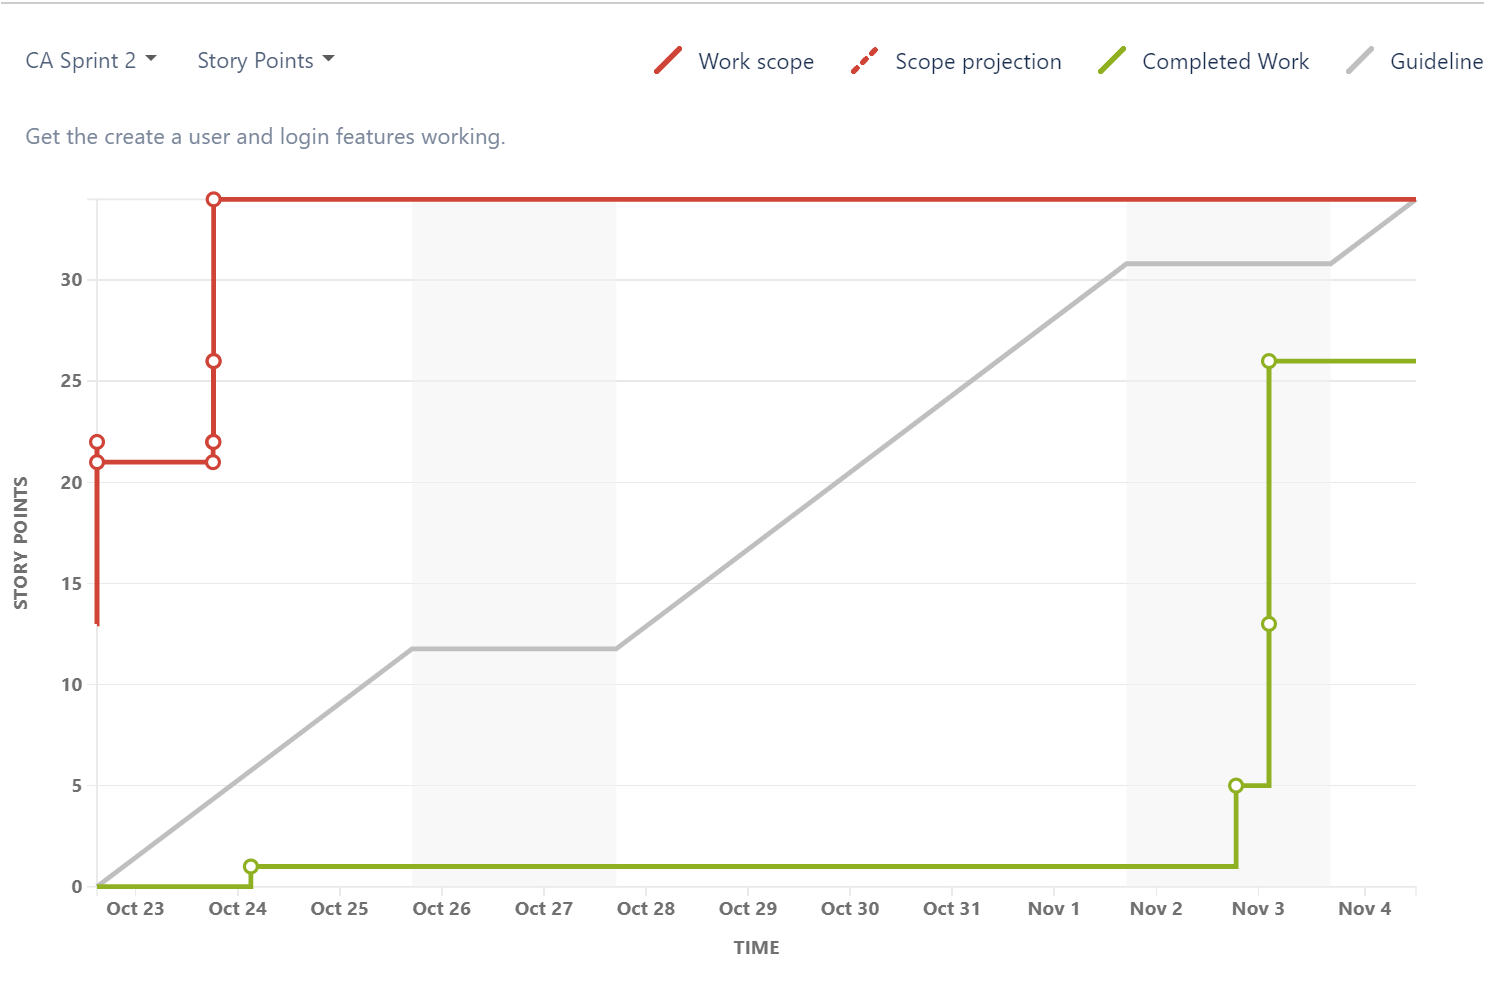
\includegraphics[width=15cm, height=10cm]{JIRA_Burnup_Chart_2.png}
         \\
					Since I didn't know how to include this in our chart,
         Here's the assigned story points versus Hours Spent 
         Assuming the Backend Split tasks almost evenly:\\
         \begin{center}
         \begin{tabular}{c c c}
         Alexander Bistagne: & 9   Story points & 29 hours\\
         Matthew Johnson:   & 8   Story Points  & 20 hours\\
         Yongsheng Cui:	      & 9   Story Points & 32 hours\\
         Weihao Ke:             & 9   Story Points & 26 hours\\
         Alfredo Vicuna:        & 11 Story Points & 40 hours
					\end{tabular}
					\end{center}
					\item To our team, a story point can be anywhere from 2 hours 30 minutes to 3 hours 30 minutes. That's a lot of variation.
					
    \end{flushleft}

\end{document}